\chapter{Method}\label{ch: ch3}%
The construction of CVs using PCA is described in detail.
Its goal is to drive an MD simulation of a chemical reaction of the form: $\text{reactants} \to \text{products}$.
\section{Illustration of the Method}
To aquire an intuition of the method first, the method will be summarized in a simplified manner. 
The state of a system can be described as a point in the descriptor space of the MLIP.
Thus, reactants states should cluster around on point in descriptor space and products states should cluster at a different point in descriptor space.
In the simulation of the reaction, the bias is applied such that the trajectory of the state wanders from the reactants cluster to the products cluster over time (see Figure \ref{fig: illustration_method_initial}). 
However the descriptor space of the MLIP  is typically very high dimensional \cite{Schaefer2025}. For example, the MLIP used in this thesis was MACE-MPA-0 and its descriptor space is 256 dimensional \cite{batatia2024foundation}.
This makes the bias application in MetaD ineffective \cite{Laio2008}. \\

Here, PCA is used to find a lower dimensional subspace (1-5 dim) \cite{Laio2008}. 
The reactants cluster and the products cluster are then projected onto the PCA subspace and the bias is applied on the subspace to get from the projected reactants to the projected products. 
Optimally, the projection is close enough such that eventually, the MD gets to the true products point (see Figure \ref{fig: illustration_method_pca}).

\begin{figure}[H]
    \centering % Zentriert die gesamte Abbildung
    \begin{subfigure}[t]{0.45\textwidth}
        \centering
        \includegraphics[width=\linewidth]{media/chapter_1/illustration_method_initial.png}
        \caption{Simplified illustration of the method. 
        The high-dimensional descriptor space is portrayed as a 2D space and the clusters are represented as points.}
        \label{fig: illustration_method_initial}
    \end{subfigure}
    \hfill % <--- WICHTIG: Schiebt die Bilder schön auseinander
    \begin{subfigure}[t]{0.45\textwidth}
        \centering
        \includegraphics[width=\linewidth]{media/chapter_1/illustration_method_pca.png}
        \caption{The PCA subspace is portrayed as a 1D space with the green line.}
        \label{fig: illustration_method_pca}
    \end{subfigure}
    \caption{General overview of the PCA-based methodology.} % <--- Hauptcaption hinzugefügt
    \label{fig: illustration_method} % <--- Label hinzugefügt, falls du im Text darauf verweisen willst
\end{figure}
\newpage
A visual overview of the construction of the CVs is shown in Figure \ref{fig: method_overview}.
\begin{figure}[h]
    \centering
    \includegraphics[width=0.8\textwidth]{media/chapter_3/method.png}
    \caption{Overview of the method: Setup of reactants and products (\cref{sec:setup_react_prod}), Construction of global descriptors (\cref{sec:global_descriptors}), PCA analysis (\cref{sec:pca_analysis}), Transformation to PCA space (\cref{sec:transform_pca}), and Construction of CVs (\cref{sec:construction_cvs}).}
    \label{fig: method_overview}
\end{figure}

\section{Setup of the Reactants and the Products}
\label{sec:setup_react_prod}
To analyze the chemical reaction following the procedure illustrated in Figure \ref{fig: method_overview}, two separate simulation cells are set up for the reactants and the products each.
The simulation cells are cubic boxes with periodic boundary conditions (PBC) and will be referred to as boxes in the following.
In the reactants box, one molecule of each reactant is placed. Additionally, a number of solvent molecules are added to the box to mimic the real environment. 
The same is done for the products box, where one molecule of each product is placed along with the same number of solvent molecules as in the reactants box.
Then, structure optimization is performed and an MD simulation is run for each box. 
This is done to get a list of frames for each box in order to obtain an "average configuration" for the reactants and the products. 

\newpage

\section{Construction of Global Descriptors}
\label{sec:global_descriptors}
Next, global descriptors are constructed to obtain a vectorial representation of the state of the system. 
The global descriptors are then calculated for each frame of the MD simulations. 
The process is as follows:

\begin{enumerate}
    \item An MLIP computes the local descriptors for each atom in each frame of the MD simulations.
    For the $i$-th frame, the local descriptor for the $j$-th atom is denoted as $\vct{G}_{i}^{(j)}$ with $\dim(\vct{G_{i}^{(j)}}) = N_{\text{features}}$.
    \item The global descriptor for the $i$-th frame is then obtained by averaging the descriptors of all atoms in that frame:
    \begin{align}
        \vct{G}_i = \frac{1}{N_{\text{atoms}}} \sum_{j=1}^{N_{\text{atoms}}} \vct{G_{i}^{(j)}} \quad \text{ with } \dim(\vct{G}_i) = N_{\text{features}}
    \end{align}
    As demonstrated by Schäfer and Kästner, global descriptors have already demonstrated to be effective in characterizing overall system states for dataset analysis and data selection tasks while maintaining differentiability and increasing computational efficiency\cite{Schaefer2025}.
    \item The global descriptor is then constructed for every frame of the MD simulation of the reactants and the list of global descriptors $\matr{G}_{\text{react}}$ for the reactants is obtained:
    \begin{align}
    \matr{G}_{\text{react}} &= ( \vct{G}_{\text{react},1}, \vct{G}_{\text{react},2}, \dots, \vct{G}_{\text{react},N_{\text{frames, react}}} )  \nonumber \\
    &\text{ with } \dim(\vct{G}_{\text{react}}) = N_{\text{frames, react}} \times N_{\text{features}} 
    \end{align}
    \item All steps are repeated for the products box. The list of global descriptors for the reactants and the products are then combined:
    \begin{align}
    \matr{G} &= ( \vct{G}_{\text{react},1}, \dots, \vct{G}_{\text{react},N_{\text{frames, react}}} , \vct{G}_{\text{prod},1}, \dots, \vct{G}_{\text{prod},N_{\text{frames, prod}}} ) \nonumber \\
    &\text{ with } \dim(\vct{G}) = (N_{\text{frames, react}} + N_{\text{frames, prod}}) \times N_{\text{features}} 
    \end{align}
\end{enumerate}

\section{PCA of the List of Global Descriptors}
\label{sec:pca_analysis}
PCA is performed on the list of global descriptors $\vct{G}$:
\subsection{Perform PCA}
\begin{enumerate}
    \item The mean of the list of global descriptors is calculated and subtracted from the list to center the data:
    \begin{align}
    \vct{\mu} &= \frac{1}{N_{\text{frames}}} \sum_{i=1}^{N_{\text{frames}}} \vct{G}_{i}  \\
    \overline{\matr{G}} &= \matr{G} - \vct{\mu} = ( \vct{G}_{\text{react},1} - \vct{\mu}, \dots, \vct{G}_{\text{prod},N_{\text{prod,frames}}} - \vct{\mu} ) 
    \end{align}
    \item Next, the SVD of the centered data is performed:
    \begin{align}
    \overline{\matr{G}} = 
    \underbrace{
    \begin{pmatrix}
        | & & | \\
        \vct{u}_1 & \dots & \vct{u}_{N_{\text{frames}}} \\
        | & & |
    \end{pmatrix}
    }_{\matr{U}}
    \underbrace{
    \begin{pmatrix}
        \sigma_1  & \dots & 0 \\
        \vdots  & \ddots & \vdots \\
        0  & \dots & \sigma_{N_{\text{features}}} \\
        0  & \dots & 0
    \end{pmatrix}
    }_{\matr{\Sigma}}
    \underbrace{
    \begin{pmatrix}
        - & \vct{v}_1^T & - \\
        & \vdots & \\
        - & \vct{v}_{N_{\text{features}}}^T & -
    \end{pmatrix}
    }_{\matr{V}^T}
    \end{align}

    $\{\sigma_i\}$ are the singular values of the data, and $\{\vct{v}_i\}$ are the corresponding singular vectors.

    \item As the singular values are ordered in descending order, the first $k$ singular vectors $\vct{v}_1, \dots, \vct{v}_k$ correspond to the directions of maximum variance in the data.
    While there is no strict theoretical guarantee that the directions of maximum variance perfectly align with the most relevant collective motions of the system, 
    relying on this assumption has proven to be effective in practice \cite{Schaefer2025} \cite{sicard:hal-00994220}. 
    Therefore, the first $k$ singular vectors are selected as principal components and form the projection matrix $\matr{V}_{PCA}$:
    \begin{align}
    \matr{V}_{\text{PCA}}^T =
    \begin{pmatrix}
        - & \vct{v}_1^T & - \\
        - & \vct{v}_2^T & - \\
        & \vdots & \\
        - & \vct{v}_k^T & -
    \end{pmatrix}
    \quad  \text{ with } \dim(\matr{V}_{\text{PCA}}) = N_{\text{features}} \times k
    \end{align}

\end{enumerate}
As a result of the PCA, the principal components $\{\vct{v}_i\}$ span the PCA space: $\operatorname{span}\{\vct{v}_i\}$.
This subspace reduces the dimensionality of the data from $N_{features}$ to $k$ while retaining as much of the variance in the data as possible.
Furthermore, with the transformation matrix $\matr{V}_{\text{PCA}}$, new data can be transformed to the PCA space.

\subsection{Transform new data to the PCA Space}
\label{sec:transform_pca}
To transform a new data point $\vct{G}_{\text{new}}$ to the PCA space, it is first centered and the projected by multiplying it with the projection matrix $\matr{V}_{\text{PCA}}$:
\begin{align}
\vct{G}_{\text{new, centered}} &= \vct{G}_{\text{new}} - \vct{\mu} \\
\vct{G}_{\text{new, PCA}} &= \matr{V}_{\text{PCA}}^T \vct{G}_{\text{new}, \text{centered}}
\end{align}
The resulting vector $\vct{G}_{\text{new, PCA}}$ is the representation of the new data point in the PCA space.


\section{Construction of CVs}
\label{sec:construction_cvs}
The obtained PCA space can be used to construct CVs.
For that, the current configuration of the system is compared to the products with the distance between their projections in the PCA space.
The idea is illustrated in Figure \ref{fig: example_pca_plot}.
\begin{figure}[h]
    \centering
    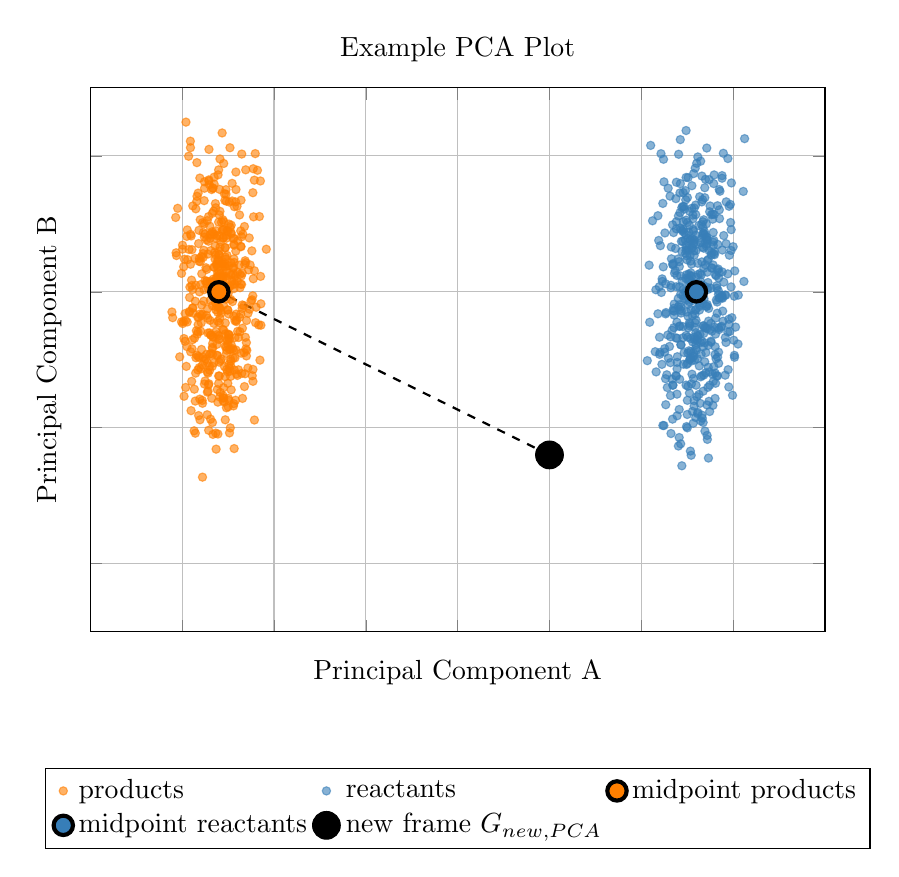
\begin{tikzpicture}
        \begin{axis}[
            % Allgemeine Einstellungen
            title={Example PCA Plot},
            xlabel={Principal Component A},
            ylabel={Principal Component B},
            grid=major,
            xmin=-0.2, xmax=0.2, % Achsenbereich anpassen
            ymin=-0.25, ymax=0.15,
            xticklabels={},
            yticklabels={},
            width=0.9\textwidth, % Breite des Plots
            height=0.7\textwidth, % Höhe des Plots
            scatter/use mapped color={draw=mapped color,fill=mapped color},
            legend style={
                cells={anchor=west},
                at={(0.5,-0.25)}, % unterhalb der Achse
                anchor=north,
                legend columns=3, % Einträge nebeneinander
            },
        ]

            % Benutzerdefinierte Farben definieren (ähnlich dem Originalbild)
            \definecolor{reactantBlue}{HTML}{377EB8}
            \definecolor{productOrange}{HTML}{FF7F00}

            % --- 1. DATENPUNKTE ---

            % Generiere Punkte für Produkte (orange, links)
            \addplot[
                only marks,
                mark=*,
                mark size=1.5pt,
                fill=productOrange,
                draw=productOrange,
                opacity=0.6, % Transparenz
                domain=0:1,
                samples=500, % Anzahl der Punkte pro Cluster
                samples y=1,
            ] ({
                % Gauss-ähnliche Verteilung (Summe von 3 Zufallszahlen ≈ Normalverteilung)
                -0.13 + 0.01*(rand+rand+rand)
            },{
                0.0 + 0.05*(rand+rand+rand)
            });
            \addlegendentry{products}

            % Generiere Punkte für Reaktanten (blau, rechts)
            \addplot[
                only marks,
                mark=*,
                mark size=1.5pt,
                fill=reactantBlue,
                draw=reactantBlue,
                opacity=0.6,
                domain=0:1,
                samples=500,
                samples y=1,
            ] ({
                0.13 + 0.01*(rand+rand+rand)
            },{
                0 + 0.05*(rand+rand+rand)
            });
            \addlegendentry{reactants}


            % --- 2. MITTELPUNKTE ---

            % Mittelpunkt Produkte (orange, links)
            \addplot[
                only marks,
                mark=*,
                mark size=3.5pt, % Größer
                fill=productOrange,
                draw=black, % Schwarzer Rand
                line width=1.5pt, % Dicker Rand
            ] coordinates {(-0.13, 0.00)};
            \addlegendentry{midpoint products}

            % Mittelpunkt Reaktanten (blau, rechts)
            \addplot[
                only marks,
                mark=*,
                mark size=3.5pt,
                fill=reactantBlue,
                draw=black,
                line width=1.5pt,
            ] coordinates {(0.13, 0.00)};
            \addlegendentry{midpoint reactants}


            % --- 3. NEUER PUNKT ---

            % Neuer Punkt (schwarz, groß)
            \addplot[
                only marks,
                mark=*,
                mark size=5pt,
                fill=black,
                draw=black,
            ] coordinates {(0.05, -0.12)};
            \addlegendentry{new frame $\vct{G}_{\text{new, PCA}}$}

            % Gestrichelte Linie vom neuen Punkt zum Mittelpunkt Produkte
            \addplot[
                dashed,
                thick,
                black,
            ] coordinates {(0.05, -0.12) (-0.13, 0.00)};
            %\addlegendentry{distance to midpoint products}



        \end{axis}
    \end{tikzpicture}
    \caption{
    Example PCA plot with 2 Principal Components (PCs). A dot in the plot represents the projection of a frame of an MD simulation to the PCA space, blue originate from the reactants MD and orange from the products MD.
    }
    \label{fig: example_pca_plot}
\end{figure}

The frames of the reactants and the products each form a cluster in the PCA space. Therefore, the proximity of a frame to a cluster can be used as an indicator of the state of the system. For example, if a frame is closer to the products cluster, it is more likely that the system is in a state that resembles the products.
A new frame of the MD simulation of the system can be projected to the PCA space as well, which is represented by the black dot in the plot. The distance from this new point to the midpoint of the products cluster (dashed line) can be used as a CV for enhanced sampling methods.
Here, multiple metrics in the PCA space are imaginable. In this work, the euclidean distance to the projection of the system in the PCA space $ \vct{G}_{current, PCA} $ to the midpoint of the products cluster $ \vct{m} $ is used as a CV:
\begin{align} \label{eq: constructed_CV}
CV\_dist \quad := \| \matr{V}_{\text{PCA}}^T \vct{G}_{\text{current}} - \vct{m} \|_2 = \| \vct{G}_{\text{current, PCA}} - \vct{m} \|_2
\end{align}
Other metrics could be implemented as well, such as using the $\|\cdot\|_1$ norm or increasing the number of PCs and then using the distance in the higher-dimensional PCA space as CV.



